% File name: datalogger/3DAQ/Documentation/Data_Transmission_Setup.tex
% Description of how data and commands will be transmitted between board and pc.
% Author: adh
% Date: Fri 24 May 2013 16:17

\documentclass[a4paper,11pt]{article}  % Standard document class
\usepackage[english]{babel}            % Set document language
\usepackage{fullpage}                  % Set up page for small margins etc

\usepackage{graphicx}                  % For including images in document
\usepackage{placeins}                  % Allows use of \FloatBarrier
% to avoid images or tables
% moving into next section
\usepackage{subfig}                    % For subfigures...

\usepackage{amsmath}                   % For improving maths/formula typesetting
\usepackage{tabularx}                  % Table changing package

\usepackage{algpseudocode}             % For producing algorithms/flowcharts
\usepackage{listings}                  % For including source code in document


% Provide command for scientific notation
\providecommand{\e}[1]{\ensuremath{\times10^{#1}}}
\providecommand{\degrees}{\ensuremath{^{\circ}}}

% Define title here:
\title{Communication and Data Transfer Protocol}
\author{James Glandular\\ jg597 \and Andrew Holt\\ ah635}
\date{24 May 2013}

\begin{document}

% generate title
\maketitle

\noindent The data logger works in 2 modes:

\begin{description}
  \item[Streaming Mode:] board is linked to computer and data is
    streamed up to the computer directly.
  \item[Standalone Mode:] board is not connected and stores data in
    EEPROM. The data is later transferred to the computer.
\end{description}

\section{Streaming Mode}

\begin{itemize}
  \item Every period, the board will send a packet of data to the
    computer.
  \item Each packet is 10 bytes long.
  \item The first 2 bytes will contain temperature data, and the third
    byte will contain humidity data. The rest will contain
    accelerometer data but not yet specifically defined.
\end{itemize}

\begin{center}
  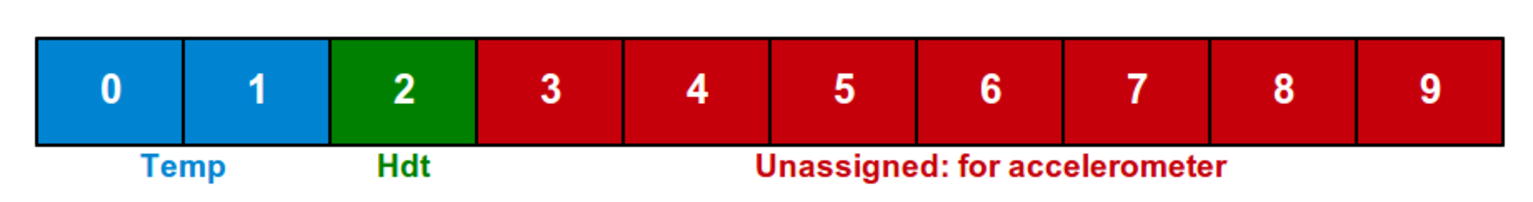
\includegraphics[width=0.8\textwidth]{Packet_diagram.pdf}
\end{center}

\section{Standalone Mode}

\begin{itemize}

\end{itemize}

\end{document}